\documentclass{article}
\usepackage{amsmath}
\usepackage{amsfonts}
\usepackage{graphicx}
\usepackage{mathtools}
\usepackage{bm}
\usepackage[margin=1in]{geometry}

\title{NEML CW}
\author{Ben James, Johns Noble}
\date{March 2025}
\begin{document}
\maketitle
\tableofcontents
\section{Introduction}

At the core of many modern machine learning algorithms is the multivariate gaussian distribution, the most common choice for modelling and estimating true data distributions. The density of this distribution requires a notion of distance between points, which is often chosen to be the Mahalanobis distance. This distance uses the Euclidean norm, and therefore is an effective choice for modelling linear data. However, true data distributions are often non-linear, and the Euclidean multivariate gaussian does not generalise well to modelling these cases because it does not make sense for a region outside the manifold to possess non-zero measure. When data lies near an embedded manifold, the choice of distance metric can be changed to better model the nonlinear nature. The Locally Adaptive Normal Distribution (LAND) \cite{arvanitidisLocallyAdaptiveNormal2016} is a method that replaces the Euclidean distance with a locally adaptive Riemannian distance that can be used to build a multivariate normal distribution for data lying on a Riemannian manifold \cite{manfredoRiemannianGeometry1992}.

Once LAND introduces the notion of a multivariate normal distribution on a manifold, distributions can be fit using maximum likelihood estimation (MLE). Numerical methods such as Monte Carlo integration and gradient-based optimisations can be used to estimate the mean and covariance of the distribution. Finally, with an estimate of the data, it becomes possible to perform a range of machine learning algorithms that would typically use the Euclidean multivariate normal, such as EM algorithms for estimating mixtures of LANDs.

In this report, we will implement and experiment with the LAND method for estimating parameters of a nonlinear distribution. More specifically, we will generate data that lies along an embedded 3D sphere, and experiment with fitting a LAND distribution to this data. We will investigate two approaches: one where the spherical nature of the manifold is known, and one where the manifold must be learned from the data.

\section{Constructing Metrics}
In order to define the idea of distances over manifolds and in order to attempt to capture local behaviour of data, we need to a Riemannian Metric which acts on tangent vectors.
The Metric $\textbf{M(x)}$ gives an inner product $\langle \textbf{u, M(x)v}\rangle$
This allows us to define geodesics on our manifold as the path which minimises the length:
$$\hat{\gamma} = \underset{\gamma}{argmin} \int_0^1\sqrt{\langle \gamma'(t),\textbf{M}(\gamma(t))
\gamma'(t)\rangle}dt,\: \gamma(0)=\textbf{x},\:\gamma(1)=\textbf{y}$$
Once we have $\hat{\gamma}$ it is natural to define our Exponential map given a $\textbf{v}\in T_\textbf{x}M$ such that $\textbf{y} =Exp_\textbf{x}(\textbf{v}) \in M$ where $\hat{\gamma}(t) = Exp_\textbf{x}(t\cdot\textbf{v})$.
We can then begin to define the $Log$ mapping as: $Log_\textbf{x}(y)=v\in T_\textbf{x}M$.
In order to calculate each geodesic, we must express solve the equation relating Christofell symbols.
This works out to be a second order differential ODE that in practice can be solved numerically.

A generalised view of thinking about the normal distribution is the distribution over a given space such that given a known mean and covariance for which we have maximum entropy.
This way of defining the normal distribution allows us to extend to non euclidean spaces.
It can be shown that given a Log map, the distribution that satisfies this is as follows:

$$p_M(\bm{x}|\bm{\mu},\bm{\Sigma}) = exp(-\frac{1}{2}\langle Log_{\bm{\mu}}(\bm{x}),
\bm{\Sigma}^{-1}Log_{\bm{\mu}}(\bm{x})\rangle)$$
We also need to make considerations on how we can learn a metric tensor so that we can define a Riemannian metric.
The most obvious thing we can do is to use a single global metric tensor such that $dist^2(\bm{x}_i, \bm{x}_j = (\bm{x}_i-\bm{x}_j)^T\bm{M}(\bm{x}_i-\bm{x}_j)$ where $M$ is symmetric and positive definite.
The issue with this is that a single global metric is never enough to capture the nonlinearity of manifolds.
We can attempt to also learn several metric tensors for different sections of data.
This involves picking a few centres $(\bm{x_1}, \bm{x_2} ... \bm{x_r})$, defining a fixed metric $\bm{M}_r$ for each data point picking the closest metric.
We can generalise this sort of approach by letting:
$$\bm{M}(\bm{x}) = \Sigma_{r=1}^R\frac{w_r(\bm{x})}{\Sigma_jw_j(\bm{x})}\bm{M}_r$$
Intuitively, we can think of the ratio of $w_i$ to be the responsibility of each centre for $\bm{x}$.
For example in the case of picking the nearest tensor, we can say that:
$$w_r(x) = \begin{cases} 1,&\|\bm{x}-\bm{x}_r\|_{\bm{M}_r}^2 \leq \|\bm{x}-\bm{x}_j\|_{\bm{M}_j}^2, \forall j \\
0,& \text{otherwise}\end{cases}$$
There are many different ways we can construct the function $\bm{M}$ which gives a metric tensors at different points on the manifold.
In hauberg et al.\cite{haubergGeometricTakeOnMetricLearning} they discuss many different philosophies and ideas for learning a metric tensor functions.
To summarise, a metric tensor is constructed using the inverse covariance of training data in a local space.
The authors of LAND decided that when constructing metric tensors, that we should only consider the diagonals of the covariance to avoid issues with overfitting and to speed up computation.
They also used for function $w_n(\bm{x}) = exp(-\frac{\|\bm{x}_n-\bm{x}\|_2^2}{2\sigma^2})$.
Defining for the $d$ value in the diagonal of $\bm{M}$ to be $$\bm{M}(\bm{x}) = (\Sigma_{n=1}^Nw_n(\bm{x})(x_{nd}-x_d)^2+\rho)^{-1}$$
The $\rho$ is here for numerical stability and $\sigma$ can be tweaked depending on the densitty and dimensions of the data.
In our experiments we begin by assuming that the data lies on a sphere so that we could use already existing Exponential and Log mappings and the metric tensor over a sphere.
We were able to write an implementation that learnt a riemannian metric using the formula above.

\section{Parametric Inference}
\label{sec:parametric_inference}
We are tasked with finding the mean and covariance matrix of the distribution and we have implemented this using numerical methods.
The objective function we are trying to maximise is as follows:
$$\underset{\bm{\mu} \in M \bm{\Sigma} \in S_{++}^D}{\text{argmin}}(\phi(\bm{\mu},\bm{\Sigma})
=\frac{1}{2N}\Sigma_{n=1}^N\langle Log_{\bm{\mu}}(\bm{x}_n),
\bm{\Sigma}^{-1}Log_{\bm{\mu}}(\bm{x}_n)\rangle
+ log(C(\bm{\mu},\bm{\Sigma}))$$
Where $C$ here is the normalisation constant of normalisation to ensure its a probability distribution.
To compute this value we require to be able to compute $E_{N(0,\bm{\Sigma})}[\sqrt{|\bm{M}Exp_{\bm{\mu}}(\bm{v})|}]$,
intuitively can be thought of as the the expectation of the volume of the manifold.
Since this is value is intractable we use monte carlo simulation techniques to be able to compute this by sampling over $N(0,\bm{\Sigma})$.
We are able to work out two grad functions for the objective, one for the mean, one for the covariance.
The grad function for the mean is in th form $-\bm{\Sigma}^{-1}(...)$.
Simply applying gradient descent with this grad function however results in unstable convergence due to the condition number of $\bm{\Sigma}$.
We end up chosing a direction which is independent from $\bm{\Sigma}$ by taking the direction to be $-\bm{\Sigma}\nabla\phi$ which can be proved to give a direction of objective function decrease.
We also must be careful with applying gradient descent over the covariance matrix.
This is because these covariance matrices must neccesarily be symmetric positive definit.
In order to ensure that this always hold we can decompose $\bm{\Sigma} = PDP^T$ and therefore $\bm{\Sigma}^{-1} = PD^{-1}P^T= (PD^{-\frac{1}{2}})(PD^{-\frac{1}{2}})^T=A^TA$
Representing the objectives with $\bm{A}$ allows us to optimise over $\bm{A}$ and ensure our covariance matricies are valid.

\section{Experiments}
\subsection{Generating Spherical Data}
For all of our experiments, we generated synthetic data points that lie along a 3D spherical manifold. We decided to use a sphere as there already exists a well-defined exponential and log mapping for this manifold. We also used the existing implementation in the \textit{pymanopt} python library.

The first step in generating the data was picking a random point on the sphere to be our target mean. Then we generated $N$ tangent vectors by sampling from a multivariate normal distribution with a target covariance. The important considerations here were preventing any tangent vectors $v$ with $\vert\vert v\vert\vert^2 > \pi$ as this would cause the mapped geodesic to wrap around the sphere, and would affect the calculations for the metric tensor. We found that a diagonal covariance of $0.7$ was a good value to prevent this from happening. To convert the sampled points to tangent vectors, we used Gram-Schmidt orthogonalisation to build an axis at the tangent point (mean) and then projected the sampled points onto this axis.

After obtaining the tangent vectors, we used the exponential mapping to map them to the sphere. This is the step that would vary depending on the manifold we are working with. The mapping from the tangent space vectors to points on the manifold can be seen in figure \ref{fig:tangent_norm}.

\begin{figure}[h]
    \centering
    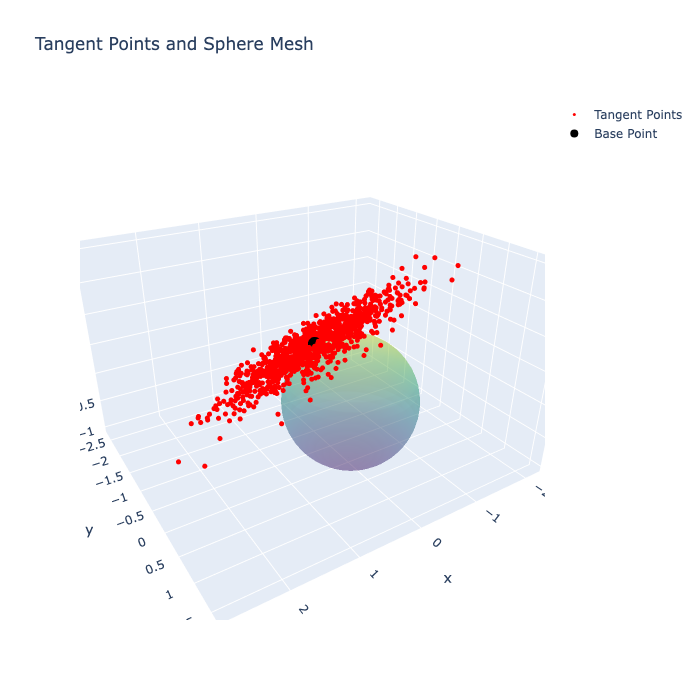
\includegraphics[width=0.4\textwidth]{plots/tangent_norm.png}
    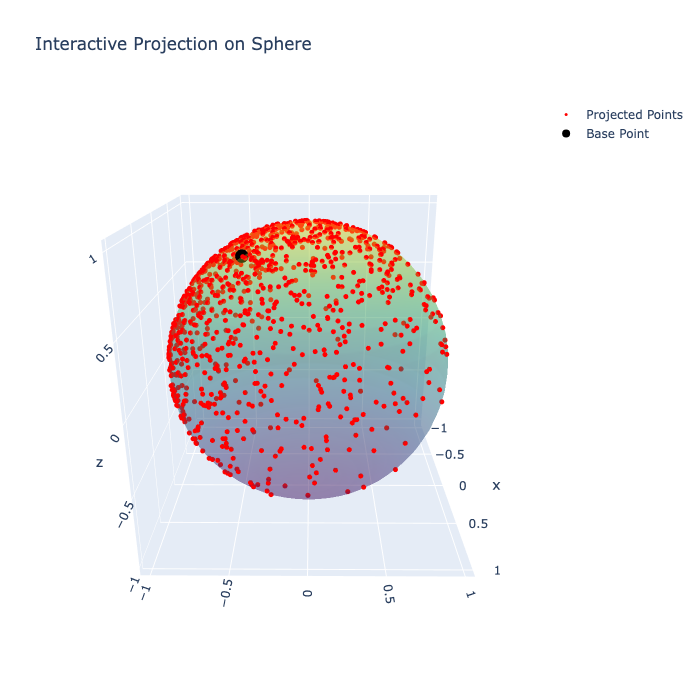
\includegraphics[width=0.4\textwidth]{plots/high_cov_proj.png}
    \caption{Tangent vectors sampled from a target normal distribution (left) and the same vectors projected onto a spherical manifold (right).}
    \label{fig:tangent_norm}
\end{figure}

\subsection{Choosing a Manifold}
The first approach we took for learning the manifold from the data was simply working under the assumption of a sphere manifold and using the existing exponential and log mappings for the sphere. We used the \textit{pymanopt} library to perform the optimisation. Whilst this does not give an insight into the performance of the LAND model on unseen data, it does provide a good starting point for understanding the LAND model and the optimisation process. Additionally, the well-defined exponential and logarithmic mappings for the sphere make computations much faster and allow us to simulate larger datasets with more iterations.

The second approach uses the metric tensor defined in the LAND paper to learn a manifold from the data. We used the same method for generating spherical data, but then attempted to learn a manifold from the same data. The initial difference that stood out was the time of computation. We implemented the exponential map using the ODE solver from the \textit{scipy} library, which was much slower than the existing exponential mapping for the sphere. This made it difficult to run the optimisation for many iterations, but we did find that with many datapoints, (high coverage of the sphere), our learned manifold often produced results similar to that of the known spherical mappings, as seen in figure \ref{fig:comparison}.

\begin{figure}[h]
    \centering
    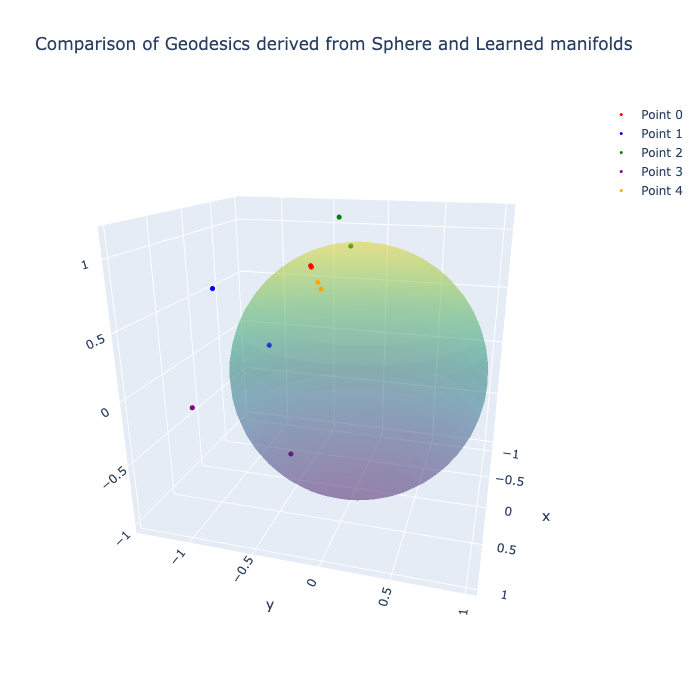
\includegraphics[width=0.6\textwidth]{plots/comparison.png}
    \caption{Pairs of points generated by the exponential map for the sphere and learned manifolds.}
    \label{fig:comparison}
\end{figure}

\subsection{Inferring Parameters}
The main part of our experiment was then attempting to learn the target distribution, given the data on the sphere. We used the MLE algorithm described in the LAND paper and in section \ref{sec:parametric_inference}. Initially we used a lower initial $\Sigma$ (diagonal) value of $0.1^2$ to aid with convergence. We found that the algorithm converged quickly for the known manifold, which is expected when all the data points are clustered closely around the target mean. Through empirical experimentation, we found the optimal hyperparameters were $\approx 100$ iterations and a step rate of $\approx 0.01$. A visual example of the convergence can be seen in figure \ref{fig:convergence}. 

\begin{figure}[h]
    \centering
    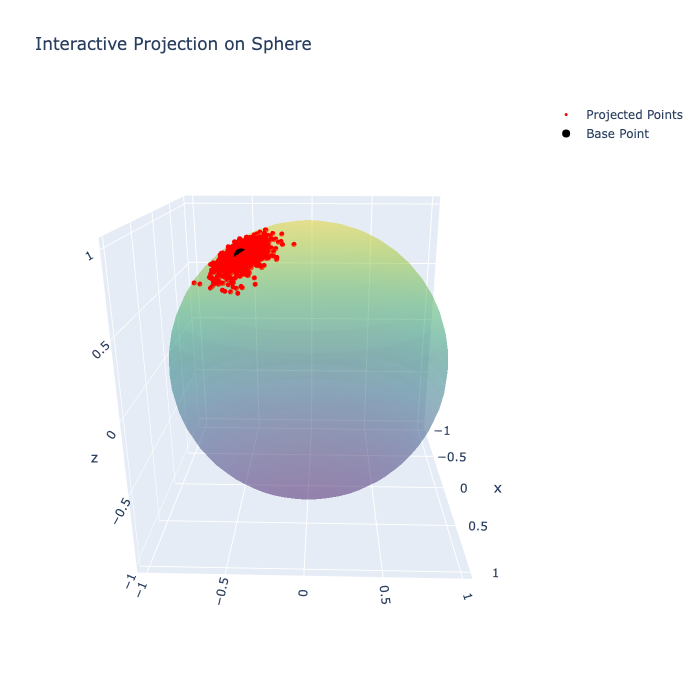
\includegraphics[width=0.4\textwidth]{plots/small_cov_proj.png}
    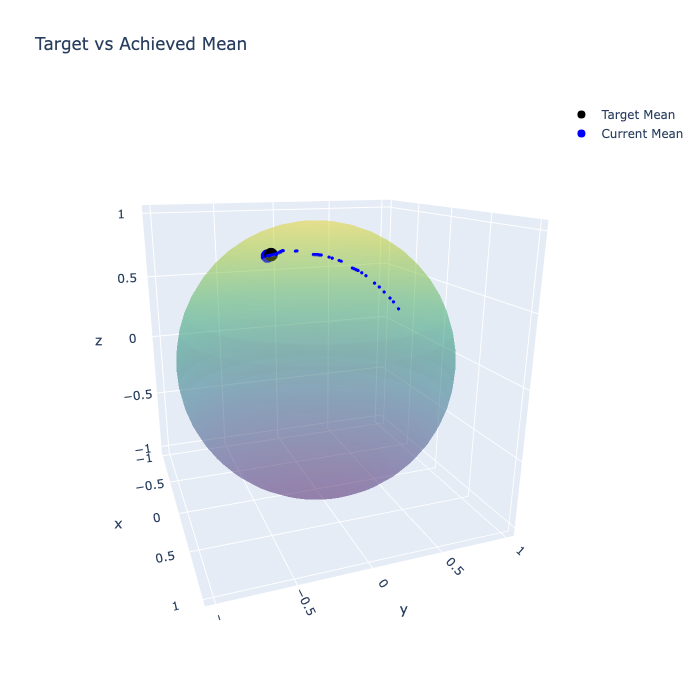
\includegraphics[width=0.4\textwidth]{plots/small_cov_no_projs.png}
    \caption{Generated distribution for $\Sigma=diag(0.1^2)$ (left) and convergence of MLE algorithm (right).}
    \label{fig:convergence}
\end{figure}

When using a higher value for $\Sigma = diag(0.7^2)$, we saw convergence was much slower. This is expected as the increased spread of data points resulted in less penalty from the $\sqrt{\vert M(exp_{\mu}(v))\vert}$ term in the objective function. Therefore, as expected, empirical tests showed that the optimal for this covariance was $\approx 300$ iterations and a step rate of $\approx 0.02$. An example of this experiment is shown in figure \ref{fig:high_convergence}.

\begin{figure}[h]
    \centering
    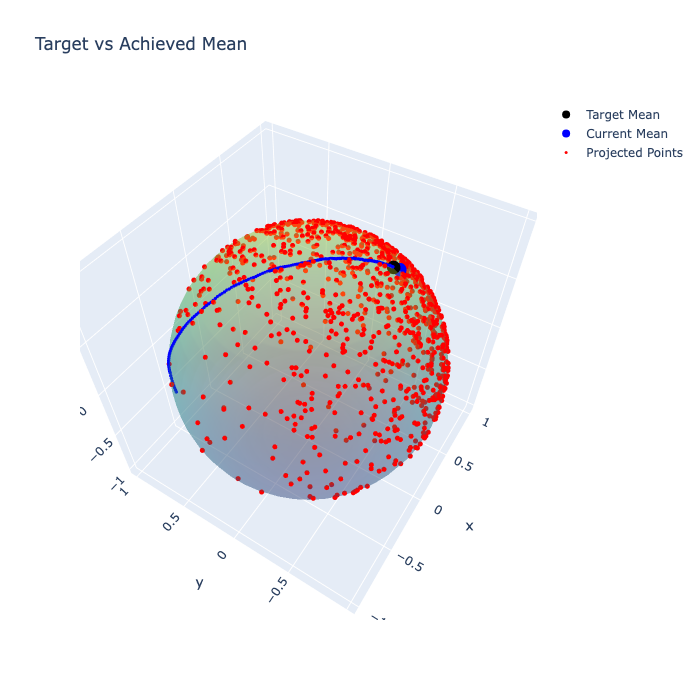
\includegraphics[width=0.6\textwidth]{plots/high_cov_with_proj.png}
    \caption{Convergence of MLE algorithm for generated data with $\Sigma=diag(0.7^2)$.}
    \label{fig:high_convergence}
\end{figure}

Finally, we attempted to apply the MLE algorithm to a learned manifold. Due to the high computational complexity of the ODE solver, we were unable to produce simulations similar to the above experiments. However, we were able to simulate a few iterations over a smaller dataset of $\approx 200$ data points. Whilst we can't verify convergence due to the low number of iterations, it's possible to see slight convergence to the correct mean. For this experiment, we increased the step rate to $0.1$ to give more pronounced results. An example of this experiment can be seen in figure \ref{fig:learned_mean}.

\begin{figure}[h]
    \centering
    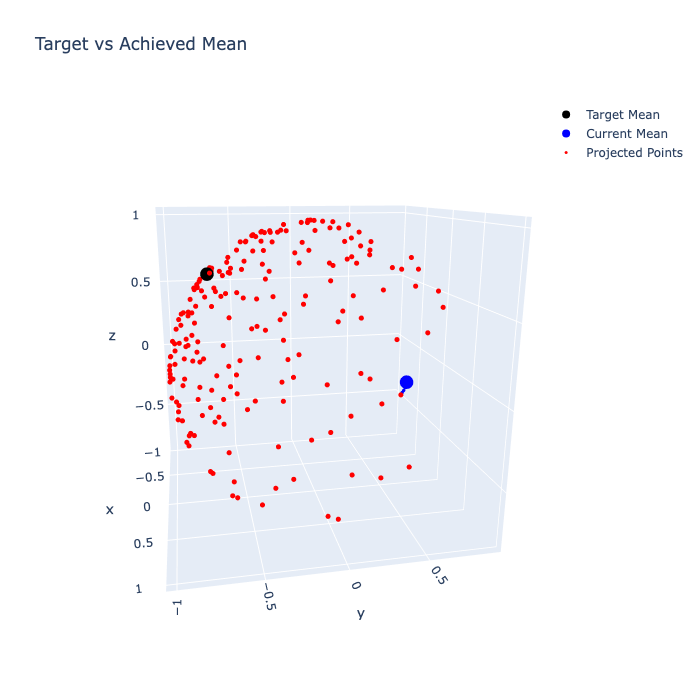
\includegraphics[width=0.6\textwidth]{plots/learned_mean.png}
    \caption{Convergence of MLE algorithm for a learned manifold on generated data with $\Sigma=diag(0.7^2)$.}
    \label{fig:learned_mean}
\end{figure}

\section{Conclusion}
We were able to show that we could perform gradient descent in the space of parameters to find an approximation for the MLE of a normal distribution on a given manifold.
We were also able given data points to learn a manifold and infer the geodesics to produce an exponential and log mapping by solving ODEs. Interestingly, we found the convergence to the target mean was, in general, much more accurate than reconstructing the target covariance matrix. We believe this is because the gradient algorithm for the mean does not depend on the covariance matrix, which can sometimes have a high condition number and cause instability in the optimisation.

Other interesting cases we found were cases where the variance of the distribution is high relative to the size of a spherical manifold.
We found in these cases that generally convergence is slower and often more inaccurate.
This should make sense since we no longer have an injective exponential map and the tails of the normal distribution are able to "wrap" back around.
This effect causes the overall distribution to look less like a normal distribution and more like a distribution with heavy tails.
We found that setting the start variance to 0.7 was a good value.
We can come up with these values by establishing bounds on the probability that a point appears over $\pi$ distance away in the tangent space.

\section{Evaluation}
If we had more time, it would certainly have been interesting to record more quantitative experimental results. Specifically about how different hyperparameters and qualities of the distribution affect the rate of convergence. Additionally, because we have implemented the algorithm for learning a manifold from data, it would be simple to experiment with more (non-spherical) data distributions and record how the algorithm performs. This would give us a better understanding of the LAND model and how it can generalise to unseen data.

Furthermore, we would have liked to better utilise hardware and accelerate the MLE algorithm. For this, we could have moved all code to use JAX constructs and use techniques such as just-in-time compilation to speed to the ODE solver. 

Finally, we would have also liked to also implement the EM algorithms from the LAND paper, and potentially apply them to real data. However, with time constraints, we were unable to do this.

\bibliographystyle{vancouver}
\bibliography{bibs/neml}

\end{document}
